\documentclass[aspectratio=169]{beamer}

\mode<presentation>
{
  \usetheme{default}
  \usecolortheme{default}
  \usefonttheme{default}
  \setbeamertemplate{navigation symbols}{}
  \setbeamertemplate{caption}[numbered]
  \setbeamertemplate{footline}[frame number]  % or "page number"
  \setbeamercolor{frametitle}{fg=white}
  \setbeamercolor{footline}{fg=black}
} 

\usepackage[english]{babel}
\usepackage[utf8x]{inputenc}
\usepackage{tikz}
\usepackage{courier}
\usepackage{array}
\usepackage{bold-extra}
\usepackage{minted}
\usepackage[thicklines]{cancel}

\xdefinecolor{dianablue}{rgb}{0.18,0.24,0.31}
\xdefinecolor{darkblue}{rgb}{0.1,0.1,0.7}
\xdefinecolor{darkgreen}{rgb}{0,0.5,0}
\xdefinecolor{darkgrey}{rgb}{0.35,0.35,0.35}
\xdefinecolor{darkorange}{rgb}{0.8,0.5,0}
\xdefinecolor{darkred}{rgb}{0.7,0,0}
\definecolor{darkgreen}{rgb}{0,0.6,0}
\definecolor{mauve}{rgb}{0.58,0,0.82}

\title[2017-10-13-lpc-testdrive]{New software for offline analysis}
\author{Jim Pivarski}
\institute{Princeton University -- DIANA}
\date{October 13, 2017}

\begin{document}

\logo{\pgfputat{\pgfxy(0.11, 7.4)}{\pgfbox[right,base]{\tikz{\filldraw[fill=dianablue, draw=none] (0 cm, 0 cm) rectangle (50 cm, 1 cm);}
\includegraphics[height=1 cm]{diana-hep-logo.png}}}}

\begin{frame}
  \titlepage
\end{frame}

% Uncomment these lines for an automatically generated outline.
%\begin{frame}{Outline}
%  \tableofcontents
%\end{frame}

%%%%%%%%%%%%%%%%%%%%%%%%%%%%%%%%%%%%%%%%%%%%%%%%%%%%%%%

%%%% START

\begin{frame}{Purpose of this talk}
\vspace{0.15 cm}
\begin{center}
\large To show you some of the software packages I've been developing \underline{so you can use them} and either get more productive or send me critical feedback.

\vspace{1 cm}
\uncover<2->{(I'm looking for beta testers.)}
\end{center}
\end{frame}

\begin{frame}{What is this software for, in the long run?}
\vspace{0.15 cm}
\large Ultimately, I and several others\footnote{Oliver Gutsche, Igor Mandrichenko (FNAL), Tanu Malik (DePaul CS), \mbox{Jean-Roch Vlimant (CalTech),\hspace{-1 cm}} Manos Karpathiotakis, Miguel Branco, Ioannis Alagiannis, Anastasia Ailamaki (EPFL/ATLAS)\ldots} want to develop a centralized service that will make plots more rapidly than you can with local skims.

\vspace{0.5 cm}
\uncover<2->{Think Google-for-HEP data. You submit a query and get a response on a short enough timescale to influence your next question.}

\vspace{0.5 cm}
\uncover<3->{We're still at the stage of testing various options, but meanwhile, I've been developing fast data access methods that you can use now, independently of any query system.}

\vspace{0.5 cm}
\uncover<4->{You can use it on your skims. (Same tools, different purpose.)}
\end{frame}

\begin{frame}{}
\begin{center}
\LARGE What I'll be showing today are various tools \\ for doing offline analysis faster.
\end{center}
\end{frame}

\begin{frame}{}
\vspace{1.2 cm}
\textcolor{darkblue}{Mental model of computing performance:} it isn't about speeding up your code, it's about {\it not slowing it down.} The mathematical function you want to compute has a fundamental speed set by the clock rate: everything else just gets in the way.

\begin{center}
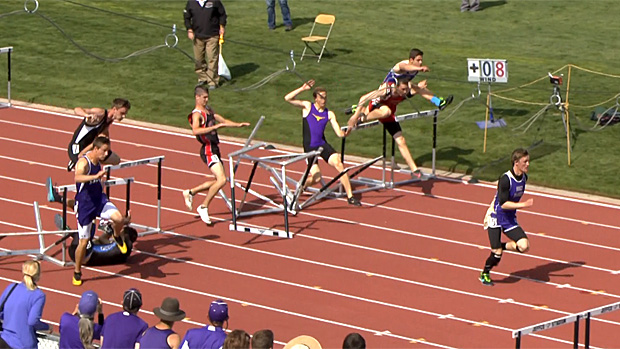
\includegraphics[width=0.7\linewidth]{hurdle9.jpg}
\end{center}
\end{frame}

\begin{frame}[fragile]{Experiment to try sometime}
\vspace{0.25 cm}
\begin{center}
\textcolor{darkorange}{\bf How long \underline{should} it take to compute an analysis function?}
\end{center}

\small
\begin{uncoverenv}<2->
\begin{minted}{python}
from time import *; from numpy import *; from math import *

pt1, pt2 = [random.normal(100, 10, int(1e6)) for i in 1, 2]
eta1, eta2 = [random.uniform(-5, 5, int(1e6)) for i in 1, 2]
phi1, phi2 = [random.uniform(-pi, pi, int(1e6)) for i in 1, 2]

start = time()
mass = sqrt(2*pt1*pt2*(cosh(eta1 - eta2) - cos(phi1 - phi2)))
end = time()

print(end - start)
\end{minted}
\end{uncoverenv}

\normalsize
\vspace{-0.75 cm}\hfill\begin{minipage}{0.35\linewidth}
\begin{uncoverenv}<3->
\begin{center}
\textcolor{darkblue}{$10^6$~events / 0.24 sec = 4.16~MHz}

\vspace{0.25 cm}
We need to get used to numbers like this.
\end{center}
\end{uncoverenv}
\vspace{0.75 cm}
\end{minipage}\hspace{0.5 cm}
\end{frame}

\begin{frame}[fragile]{Experiment to try sometime: hardcore version}
\vspace{0.1 cm}
\scriptsize
\begin{minted}{python}
import ctypes
import os

open("little-c-function.c", "w").write("""
#include "math.h"

void computemass(double* pt1, double* eta1, double* phi1,
                 double* pt2, double* eta2, double* phi2,
                 double* mass) {
  int i;
  for (i = 0;  i < (int)1e6;  i++)
    mass[i] = sqrt(2*pt1[i]*pt2[i]*(cosh(eta1[i] - eta2[i]) - cos(phi1[i] - phi2[i])));
}
""")
os.system("gcc -O3 -shared -fPIC little-c-function.c -o little-c-function.so")

computemass = ctypes.cdll.LoadLibrary("little-c-function.so").computemass
output = numpy.empty(int(1e6))

start = time()
computemass(*[x.ctypes.data_as(ctypes.POINTER(ctypes.c_double))
                                   for x in pt1, eta1, phi1, pt2, eta2, phi2, output])
end = time()

print(end - start)
\end{minted}
\normalsize
\vspace{-8 cm}\hfill\begin{minipage}{0.35\linewidth}
\begin{uncoverenv}<2->
\begin{center}
Hardcore is not much faster:

\textcolor{darkblue}{$10^6$~events / 0.203 sec = 4.9~MHz}
\end{center}
\end{uncoverenv}
\vspace{8 cm}
\end{minipage}
\end{frame}

\begin{frame}{}
\vspace{1 cm}
\begin{center}
\large If you're computing considerably fewer than 5~million masses per second, most of your computer's time is spent doing something other than physics.
\end{center}

\vspace{0.5 cm}
\begin{itemize}
\item<2-> Usually, there's a good reason: loading data or managing complexity.
\end{itemize}
\end{frame}

\begin{frame}{Loading data: cold to warm cache}
\vspace{0.25 cm}
\begin{center}
\only<1>{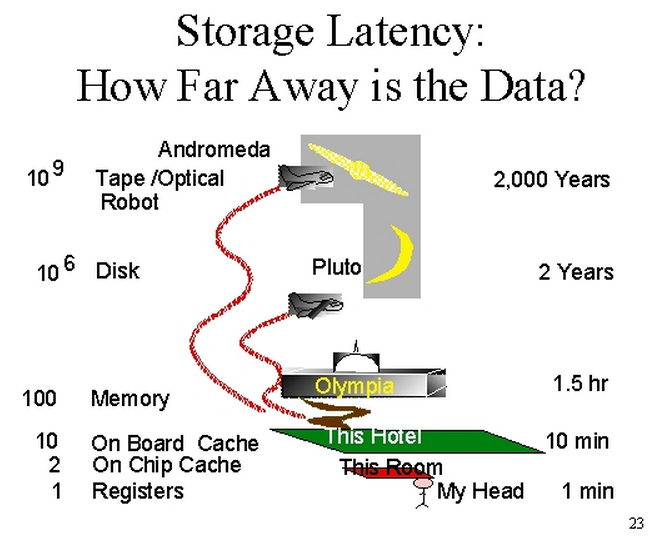
\includegraphics[width=0.67\linewidth]{storage-latency-how-far-away-is-the-data.png}}
\only<2>{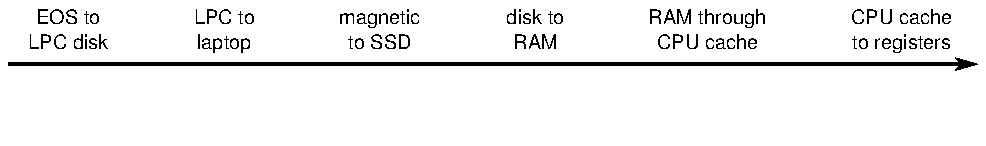
\includegraphics[width=\linewidth]{what-you-do-1.pdf}}
\only<3>{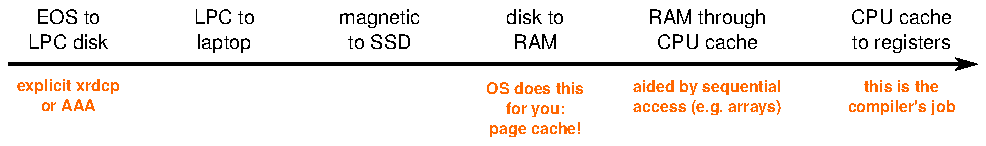
\includegraphics[width=\linewidth]{what-you-do-2.pdf}}
\end{center}
\end{frame}

\begin{frame}{Managing complexity}
\vspace{0.5 cm}
\begin{itemize}\setlength{\itemsep}{0.4 cm}
\item Python is one of the slowest languages available, and yet I used it for the high-speed mass calculation.
\item<2-> Actually, I just set up the calculation in Python and let it run in compiled code (Numpy). Python makes you think in terms of ``slow control'' and ``fast math.''
\item<3-> The slow, dynamic, abstract programming model has value: it reaches out to match the way we (humans) think.
\item<4-> But once we've specified a mathematical task, we want it to get out of the way.
\end{itemize}
\end{frame}

\begin{frame}{Getting the data at full speed}
\vspace{0.5 cm}
ROOT data are stored in an efficient format--- arrays like the ones in the high-speed mass calculation. (TBranches chopped up into TBaskets\ldots)

\vspace{1 cm}
\uncover<2->{\textcolor{darkblue}{But {\tt TTree::GetEntry} is slow:} pieces of each array are spliced into local variables each time it's called. (Also, it thwarts vectorization, has virtual function calls\ldots)}

\vspace{1 cm}
\uncover<3->{Accessing the data without {\tt GetEntry} is an order of magnitude faster.

\vspace{0.2 cm}
We're adding a method to ROOT \only<3>{6.12 (next version)}\only<4>{\xcancel{6.12 (next version)} 6.14 (next summer)} to dump data directly into Numpy arrays.}
\end{frame}

\begin{frame}{Illustration using NanoAOD decompression rate studies}
\begin{center}
\textcolor{darkblue}{\large Hint: vertical scale on right is 30$\times$ higher, reaches 0.5~MHz}
\end{center}

\begin{columns}
\column{0.45\linewidth}
\mbox{ } \hfill Reading through {\tt GetEntry} \hfill \mbox{ }

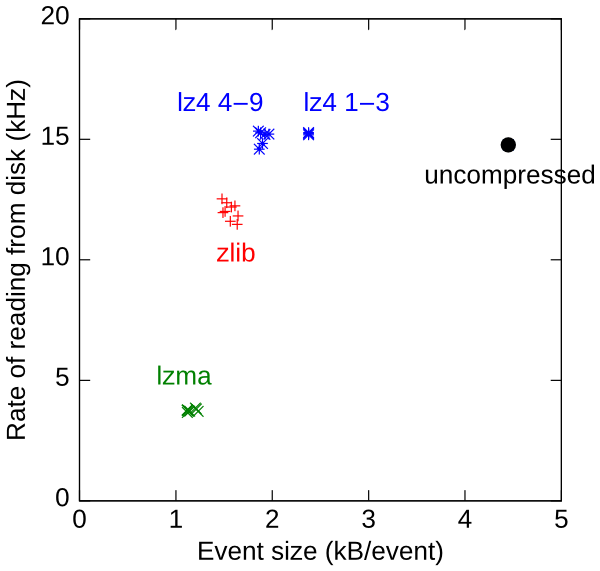
\includegraphics[width=\linewidth]{read.png}

\column{0.45\linewidth}
\mbox{ } \hfill New ROOT-to-Numpy method \hfill \mbox{ }

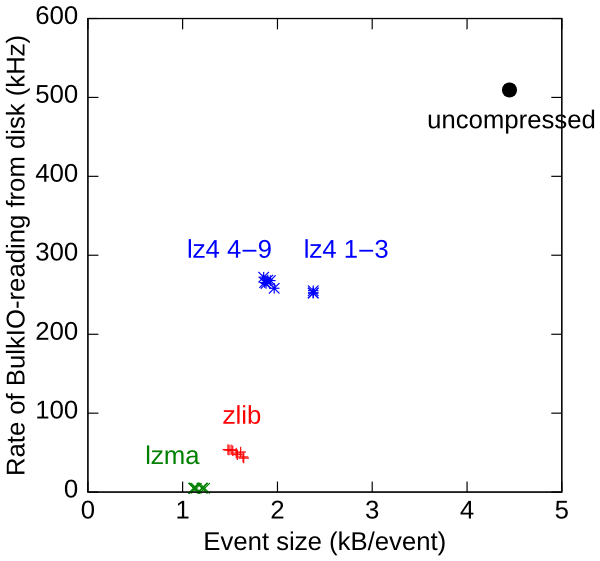
\includegraphics[width=\linewidth]{bulk.png}

\end{columns}
\end{frame}

\begin{frame}{Next summer is a long time to wait\ldots}
\vspace{0.5 cm}
So I wrote this access method in pure Python+Numpy:

\begin{center}
\href{https://github.com/scikit-hep/uproot}{\textcolor{blue}{\Large https://github.com/scikit-hep/uproot}}
\end{center}

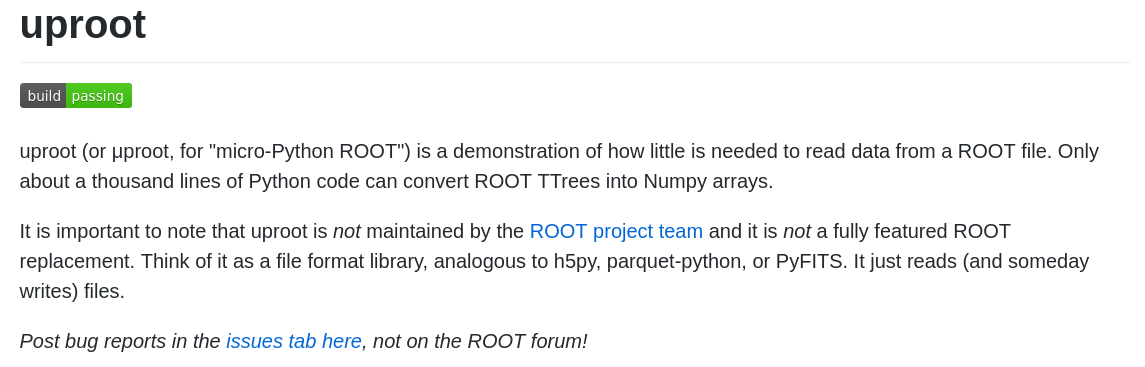
\includegraphics[width=\linewidth]{uproot.png}

\begin{center}
\Large \textcolor{red}{\tt pip install uproot --user}
\end{center}
\end{frame}

\begin{frame}{But\ldots\ Python is slow!}
\vspace{0.4 cm}
{\large If you're reading a reasonably large file (GB+), most of the time is spent in a Numpy call, not Python.}

\vspace{0.3 cm}
\begin{uncoverenv}<2->
\begin{tabular}{l c c c}
& \underline{Time to open file}$^{\mbox{\scriptsize *}}$ & & \\
C++/{\tt GetEntry} & 0.50 sec & & \\
Python/uproot & 0.03 sec & & \\
& & & \\
 & \underline{Time to read file} & \underline{Event rate} & \underline{Data rate} \\
C++/{\tt GetEntry} & 4.62 sec & 1.9 MHz & \textcolor{white}{0}230 MB/sec \\
Python/uproot & 0.93 sec & 9.2 MHz & 1160 MB/sec \\
& & & \\
& \underline{Time to read 1 branch} & \underline{Event rate} & \underline{Data rate} \\
C++/{\tt GetEntry} & 0.256 sec & \textcolor{white}{0}33 MHz & \textcolor{white}{0}260 MB/sec \\
Python/uproot & 0.064 sec & 133 MHz & 1020 MB/sec
\end{tabular}

\vspace{0.5 cm}
{\scriptsize $^{\mbox{\scriptsize *}}$from \href{https://indico.cern.ch/event/567550/contributions/2628878/}{\textcolor{blue}{Jakob Blomer's 2017 ACAT talk}} about ROOT performance, 1 GB uncompressed, flat table from LHCb.}
\end{uncoverenv}

\vspace{-6.6 cm}\hfill\begin{minipage}{0.3\linewidth}
\begin{uncoverenv}<3->
\begin{center}
\large
\textcolor{darkblue}{about 5$\times$ faster than C++/{\tt GetEntry}}

\vspace{0.1 cm}
\textcolor{darkblue}{(new method in ROOT 6.14 is 30$\times$)}
\end{center}
\end{uncoverenv}
\vspace{6.6 cm}
\end{minipage}
\end{frame}

\begin{frame}{But\ldots\ Python's GIL prevents parallelization, right?}
\vspace{0.4 cm}
{\large Python's Global Interpreter Lock (GIL) slows down parallelization of {\it Python statements,} but not external calls that release this lock.}

\vspace{0.35 cm}
\textcolor{darkblue}{uproot scales up to about 30 threads \mbox{(Knight's Landing with 128 threads shown below).\hspace{-1 cm}}}

\vspace{0.35 cm}
\begin{columns}
\column{0.4\linewidth}
\mbox{ } \hfill scaling of whole-file reading \hfill \mbox{ }

\vspace{0.2 cm}
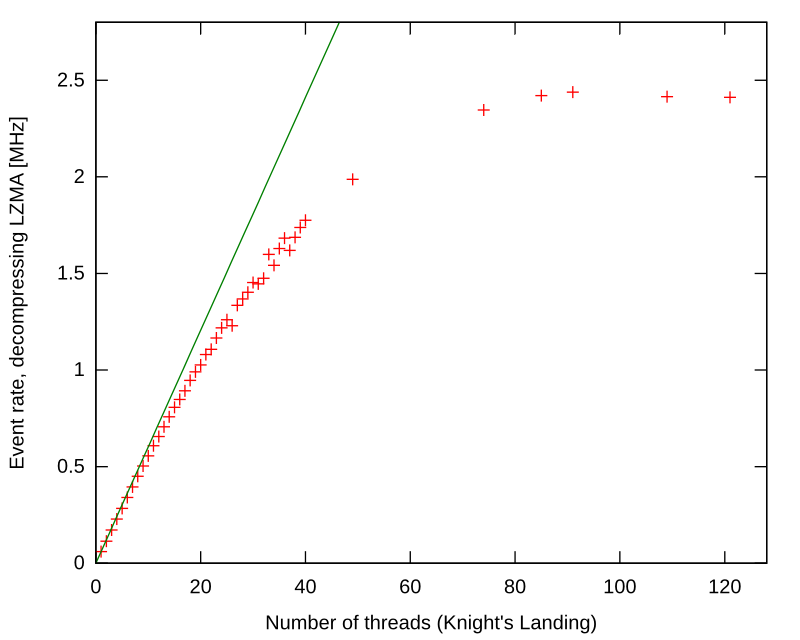
\includegraphics[width=\linewidth]{uproot-scaling.png}

\column{0.4\linewidth}
\mbox{ } \hfill scaling of single-branch reading \hfill \mbox{ }

\vspace{0.2 cm}
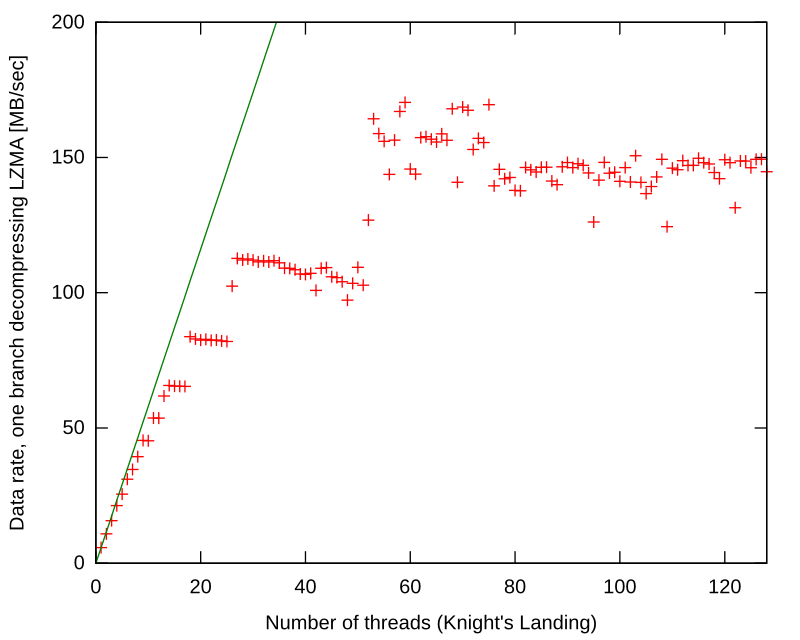
\includegraphics[width=\linewidth]{uproot-scaling-2.png}
\end{columns}
\end{frame}

\begin{frame}{}
\begin{center}
\LARGE So let's try it out!
\end{center}
\end{frame}


\end{document}
